\section{Opgave 3: På opdagelse igennem underrum i $\mathbb{R}^5$}
\NiceMatrixOptions{cell-space-limits = 3pt}

I $\mathbb{R}^5$ er givet vektorerne $a_1 = (0,1,2,2,0)$, $a_2 = (1,1,4,0,0)$, $a_3 = (1,2,6,2,1)$, $a_4 = (-1,2,2,6,-1)$, $a_5 = (2,-2,0,1,0)$ og $a_6 = (-2,-2,1,0,0)$.



\subsection{Vis at \(a_1, a_2\) og $a_3$ udspænder et 3-dimensionalt rum $\mathbf{U}$ og at \(a_4 \in \mathbf{U}\). Skriv $a_4$ som en linearkombination af $a_1, a_2$ og $a_3$.}
For at vise at de tre vektorer udspænder et 3-dimensionalt rum vises det først at de 3 vektorer ikke kan være lineærkombinationer af hindanden ved at vise at man kan lave en lineærkombination af de 3 vektorer der giver 0-vektoren. Dette gøres ved at lave en matrix af de 3 vektorer med en 0-søjle sat til sidst. Hvis man så lave en trappematrix af denne skal den vise at de tre vektorer skal bruges til at lave 0-vektoren.

\begin{align}
eMe_{1,2,3,0} =
    \bnmatrix
0 & 1 & 1 & 0 
\\
 1 & 1 & 2 & 0 
\\
 2 & 3 & 6 & 0 
\\
 2 & 0 & 2 & 0 
\\
 0 & 0 & 1 & 0 
    \enmatrix
    \xrightarrow[]{} \textbf{trap(M)} =
    \bnmatrix
    1 & 0 & 0 & 0 
\\
 0 & 1 & 0 & 0 
\\
 0 & 0 & 1 & 0 
\\
 0 & 0 & 0 & 0 
\\
 0 & 0 & 0 & 0 
    \enmatrix
\end{align}

Det ses at 0-vektoren er en lineærkombination af de 3 vektorer og dermed er de ikke lineærkombationer af hinaden. Da det er 3 vektorer som nu er vist er lineært uafhænige betyder det at de derfor udspænder et 3-dimensionelt rum, da der er 3 af dem.

For at vise at $a_4$ er en lineærkombination af de 3 andre vektorer laves en matrix igen med de 3 vektorer bare nu med 0-vektoren erstattet af $a_4$-vektoren og denne reduceres til en trappematrix og skulle dermed være en lineærkombination af dem.

\begin{align}
eMe_{1,2,3,4} =
    \bnmatrix 
    0 & 1 & 1 & -1 
\\
 1 & 1 & 2 & 2 
\\
 2 & 3 & 6 & 2 
\\
 2 & 0 & 2 & 6 
\\
 0 & 0 & 1 & -1 
    \enmatrix
    \xrightarrow[]{} \textbf{trap(M)} =
    \bnmatrix
1 & 0 & 0 & 4 
\\
 0 & 1 & 0 & 0 
\\
 0 & 0 & 1 & -1 
\\
 0 & 0 & 0 & 0 
\\
 0 & 0 & 0 & 0 
    \enmatrix
\end{align}
Det ses at $a_4$ er en lineærkombination med formen
\begin{align}
    4\cdot a_1 + 0 \cdot a_2 + (-1) \cdot a_3 = a_4 
\end{align}

\newpage
\subsection{Vis at der findes en ortonormal basis \( (q_1, q_2, q_3) \)for $\mathbf{U}$. Angiv en sådan basis som en linearkombination af $a_1, a_2$ og $a_3$}

For at lave ortonomale baser bruges Gram Schmidt's algoritme\footnote{E-note: 15.19}. Den siger at man først laver $q_1$ ud fra $a_1$ divideret med dens længde. Dernæst laver man $q_2$ ud fra $a_2$ hvor man trækker projektionen af $a_2$ ned på $q_1$ og dividere den med længden af den for at sætte dens længde til 1. Til sidst findes $q_3$ ved at trække $a_3$ fra projektionen af $a_3$ ned på $q_1$ og projektionen ned på $q_2$.
\begin{align}
    q_1 = \dfrac{a_1}{|a_1|} = \dfrac{a_1}{\sqrt{a_1 \bullet a_1}} =
\bnmatrix 
0 
\\
 \nicefrac13 
\\
 \nicefrac23
\\
 \nicefrac23 
\\
 0 
\enmatrix 
\end{align}
Så laves $q_2$ ud fra en hjælpevektor $w_2$
\begin{align}
    w_2 = a_2 - proj(a_2, q_1) = a_2 - (a_2 \bullet q_1) \cdot q_1 
\end{align}
\begin{align}    w_2 = 
\bnmatrix
1 
\\
 1 
\\
 4
\\
 0 
\\
 0 
    \enmatrix
    -
    (\dfrac{7}{3}) \cdot 
    \bnmatrix
    0 
\\
 \nicefrac13
\\
 \nicefrac23 
\\
 \nicefrac23 
\\
 0 
    \enmatrix
    =
    \bnmatrix
    1 
\\
 0 
\\
 2 
\\
 -2 
\\
 0 
\enmatrix
\\
q_2 = \dfrac{w_2}{|w_2|} = 
\bnmatrix 
\nicefrac13
\\
 0 
\\
 \nicefrac23 
\\
 -\nicefrac23
\\
 0 
\enmatrix
\end{align}

Til sidst $q_3$
\begin{align}
    w_3 = a_3 - proj(a_3,q_2)- proj(a_3,q_1) = 
    \bnmatrix
    0 
\\
 0 
\\
 0 
\\
 0 
\\
 1
    \enmatrix
\end{align}
\begin{align}
    q_3 = \dfrac{w_3}{|w_3|} = 
    \bnmatrix
        0 
\\
 0 
\\
 0 
\\
 0 
\\
 1
    \enmatrix
\end{align}

For at vise at basis er en linearkombination laves det samme som opgave a hvor $a_4$ laves som en linearkombination af de andre vektorer. Det vil sige at der laves en matrix med de 3 a-vektorer med q-vektoren til højre og den reduceres. Så ender man med $q_1$ til $q_3$ bygget op.
\begin{align}
    &q_1 = \dfrac{1}{3} \cdot a_1\\
    &q_2 = -\dfrac{1}{3} \cdot a_1 + \dfrac{1}{3} \cdot a_2\\
    &q_3 = - 1 \cdot a_1 - 1 \cdot a_2 + 1 \cdot a_3
\end{align}

\subsection{Gør rede for at $a_5$ og $a_6$ tilhører det ortogonale komplement $\mathbf{U}^{\bot}$ til $\mathbf{U}$, og redegør for at den forrige spørgsmål omtalte basis for $\mathbf{U}$ kan udvides til en ortonormal basis \(q=(q_1,q_2,q_3,q_4,q_5)\) for $\mathbb{R}^5$}

Hvis $a_5$ skal være det ortogonale komplement til $\mathbf{U}$ betyder det at hvis man prikker $a_1$, $a_2$ og $a_3$ med $a_5$ skal det give 0-vektoren. Dette kan forkortes til at man laver en matrice af $a_1$, $a_2$ og $a_3$ som søjler.
\begin{align}
eMe_{1,2,3} =
    \bnmatrix
0 & 1 & 1
\\
 1 & 1 & 2 
\\
 2 & 3 & 6
\\
 2 & 0 & 2
\\
 0 & 0 & 1
    \enmatrix
\end{align}
Dernæst transpornerer man dem for at når man ganger $a_5$ og $a_6$ med matricen er det ligesom at prikke med hver af vektorerne. Dette ses i maple appendiks 3.1 til 3.4.
\begin{align}
    eMe_{1,2,3}^T \cdot a_5 = \mathbf{0} \\
    eMe_{1,2,3}^T \cdot a_6 = \mathbf{0}
\end{align}

Det ses yderligere at $a_5$ og $a_6$ er ortogonale på hinanden. Dette ses ved at prikke de 2 vektorer på hinanden.
\begin{align}
    a_5 \bullet a_6 = 0
\end{align}
Det vil sige at når $a_5$ og $a_6$ er ortogonale på de resterende basis og samtidig er ortogonale på hinanden betyder det at de kan laves om til ortogonale baser med Gram Schmidt i maple. Dermed opnås den ortogonale basis $Q$.
\begin{align}
    Q=\left(
    \bnmatrix
    0\\\nicefrac13\\\nicefrac23\\\nicefrac23\\0
    \enmatrix,
    \bnmatrix
    \nicefrac13\\0\\\nicefrac23\\-\nicefrac23\\0
    \enmatrix,
    \bnmatrix
    0\\0\\0\\0\\1
    \enmatrix,
    \bnmatrix
    \nicefrac23\\-\nicefrac23\\0\\\nicefrac13\\0
    \enmatrix,
    \bnmatrix
    -\nicefrac23\\-\nicefrac23\\\nicefrac13\\0\\0
    \enmatrix
    \right)
\end{align}
\newpage
Lad nu $f:\mathbb{R}^5 \xrightarrow{} \mathbb{R}^5$ være en lineær afbildning for hvilken $a_1$ og $a_2-a_1$ er en egenvektorer hørende til egenværdier $\lambda_1 =1$ henholdsvis $\lambda_2 = -1$, således at $f(a_3) = a_4$ og $\text{ker}(f) = \mathbf{U}^{\bot}$.

\subsection{Bestem afbildningsmatricen for $f$ med hensyn til basen $q$, og gør rede for at $f$ er \textit{isometrisk} (vinkel- og længdebevarende) på $\mathbf{U}$, men ikke på $\mathbb{R}^5$}
Vi har fået noget information som gør at vi kan lave 5 ligninger som kan give os afbildningsmatricen. 
Først har vi fået at vide at det ortogonale komplement i q-basen skal være kernen for denne matrice. Det vil sige at $a_5$ og $a_6$ overført til q-basen skal være kernen og hvis de prikkes med matricen skal det give en 0-vektor. Derfor skal $a_5$ og $a_6$ skiftes til q-basis med en basisskiftematrice. Denne matrice er heldigvis fundet tidligere ved at vi har fundet, ved hjælp af gram-schmidt, en matrice som er opbygget af q-søjlerne. Denne matrice er en basisskiftematrice fra q-basis til e-basis og hedder derfor $eFq$. Denne skal derfor inverteres for at få fra e til q. 
\begin{align}
    eFq =
\bnmatrix
0 & \nicefrac{1}{3} & 0 & \nicefrac{2}{3} & -\nicefrac{2}{3} 
\\
\nicefrac{1}{3} & 0 & 0 & -\nicefrac{2}{3} & -\nicefrac{2}{3} 
\\
\nicefrac{2}{3} & \nicefrac{2}{3} & 0 & 0 & \nicefrac{1}{3} 
\\
\nicefrac{2}{3} & -\nicefrac{2}{3} & 0 & \nicefrac{1}{3} & 0 
\\
0 & 0 & 1 & 0 & 0 
\enmatrix
\end{align}
\begin{align}
    qa_5 = eFq^{-1} \cdot a_5 = \bnmatrix
    0\\0\\0\\3\\0
    \enmatrix\\
    qa_6 = eFq^{-1} \cdot a_6 = \bnmatrix
    0\\0\\0\\0\\3
    \enmatrix
\end{align}
\begin{align}
    qMq \cdot qa_5 = \mathbf{0} \xrightarrow{} \bnmatrix
    f&f&f&f&f\\f&f&f&f&f\\f&f&f&f&f\\f&f&f&f&f\\f&f&f&f&f 
    \enmatrix
    \cdot \bnmatrix
    0\\0\\0\\3\\0
    \enmatrix
    = \bnmatrix
    0\\0\\0\\0\\0
    \enmatrix
\end{align}
Derfor skal 4 søjle i afbildningsmatricen være en sølje på rene nuller.

Det samme sker for $qa_6$
\begin{align}
    qMq \cdot qa_6 = \mathbf{0} \xrightarrow{} \bnmatrix
    f&f&f&f&f\\f&f&f&f&f\\f&f&f&f&f\\f&f&f&f&f\\f&f&f&f&f 
    \enmatrix
    \cdot \bnmatrix
    0\\0\\0\\0\\3
    \enmatrix
    = \bnmatrix
    0\\0\\0\\0\\0
    \enmatrix
\end{align}
Derfor er 5 søjle kun rene nuller.
\begin{align}
    qMq= \bnmatrix
    f&f&f&0&0\\f&f&f&0&0\\f&f&f&0&0\\f&f&f&0&0\\f&f&f&0&0 
    \enmatrix
\end{align}
Det vides også at, ud fra egenværdien og egenvektorne at hvis $qa_1$ ganges med afbildningsmatricen skal det give egenvektoren ud ganget med egenværdien som er 1, dvs den skal give sig selv.
\begin{align}
    qa_1 = eFq^{-1} \cdot a_1 = \bnmatrix
    3\\0\\0\\0\\0
    \enmatrix
\end{align}
\begin{align}
    qMq \cdot qa_1 = qa_1  \xrightarrow{} \bnmatrix
    f&f&f&0&0\\f&f&f&0&0\\f&f&f&0&0\\f&f&f&0&0\\f&f&f&0&0 
    \enmatrix \cdot \bnmatrix
    3\\0\\0\\0\\0
    \enmatrix = 
    \bnmatrix
    3\\0\\0\\0\\0
    \enmatrix
\end{align}
Derfor skal den første søjles første række være 1 og resten af søjlen skal være 0. 
Samtidig er det også blevet opgivet at $qa_2-qa_1$ er egenvektorer og skal give sig selv negativt når den ganges med afbildningsmatrix.
\begin{align}
    qa_2 = eFq^{-1} \cdot a_2 = \bnmatrix
    3\\3\\0\\0\\0
    \enmatrix \\
    qa_2-qa_1 = \bnmatrix
    0\\3\\0\\0\\0
    \enmatrix
\end{align}
\begin{align}
    qMq \cdot qa_2 = -qa_2  \xrightarrow{} \bnmatrix
    f&f&f&0&0\\f&f&f&0&0\\f&f&f&0&0\\f&f&f&0&0\\f&f&f&0&0 
    \enmatrix \cdot \bnmatrix
    0\\3\\0\\0\\0
    \enmatrix = 
    \bnmatrix
    0\\-3\\0\\0\\0
    \enmatrix
\end{align}
Herfra ses det at anden række i første søjle skal være -1 og resten af søljen skal være 0.
\begin{align}
    qMq= \bnmatrix
    1&0&f&0&0\\0&-1&f&0&0\\0&0&f&0&0\\0&0&f&0&0\\0&0&f&0&0 
    \enmatrix
\end{align}
For at finde den sidste række bruges det sidste information som gives. Dette er at $f(a_3) = a_4$. Dette skal foregå i q-basis.
For så at få $qa_3$ og $qa_4$ gøres.
\begin{align}
    qa_3 = eFq^{-1} \cdot a_3 = \bnmatrix
    6\\3\\1\\0\\0
    \enmatrix
    \\
    qa_4 = eFq^{-1} \cdot a_4 = \bnmatrix
    6\\-3\\-1\\0\\0
    \enmatrix
\end{align}
Derfor kan man, ud fra informationen om at $f(qa_3)=qa_4$, se at den sidste søjle i $qMq$ skal være en søjle bestående af 0 og et minus 1 i midten.
\begin{align}
    qMq= \bnmatrix
    1&0&0&0&0\\0&-1&0&0&0\\0&0&-1&0&0\\0&0&0&0&0\\0&0&0&0&0 
    \enmatrix
\end{align}
Det ses at for at afbildningsmatricen $qMq$ kun er isometrisk på underummet $\mathbf{U}$, betyder det at længden og for en vektor og vinklen mellem 2 vektorer vil være det samme før og efter den er blevet afbilledet. 
Det kan ses på matricen at de sidste 2 søjler er 0-søjler. Dette betyder at hvis en vektor har en større dimension end 3 vil dens nederste værdier blive lavet om til 0 og derfor vil længden og vinklen ikke være ens. Dette kan også ses i maple hvor der laves 4 vektorer med hhv. dimensionen 3 og dimensionen 5 og dermed er i $\mathbf{U}$ og i $\mathbb{R}^5$. Se i maple appendiks 4.9 til 4.10.

\subsection{Bestem afbildningsmatricen for $f$ med hensyn til standardbasen$e$ for $\mathbb{R}^5$, og vis den er symmetrisk}

For at lave $qMq$ om til $eMe$ skal der bruges en basisskiftematrix som ganges på begge sider af $qFq$ hvor den ene side er inverteret. Her er klart at se at matricen $eFq$ kan bruges, da dette er en basisskiftematrix fra q til e\footnote{E-note 12.34}. Derfor vil ligningen være:
\begin{align}
    qFe \cdot qMq \cdot qFe^{-1} = eMe
\end{align}

Det ses med det samme at denne matrix er symmetrisk, da værdierne er ens over diagonalen. Det kan også testes ved at transponere den og se om den er ens med den originale\footnote{E-note 15.8}. Dette passer og derfor er den symmetrisk. Se maple appendiks 5.2.

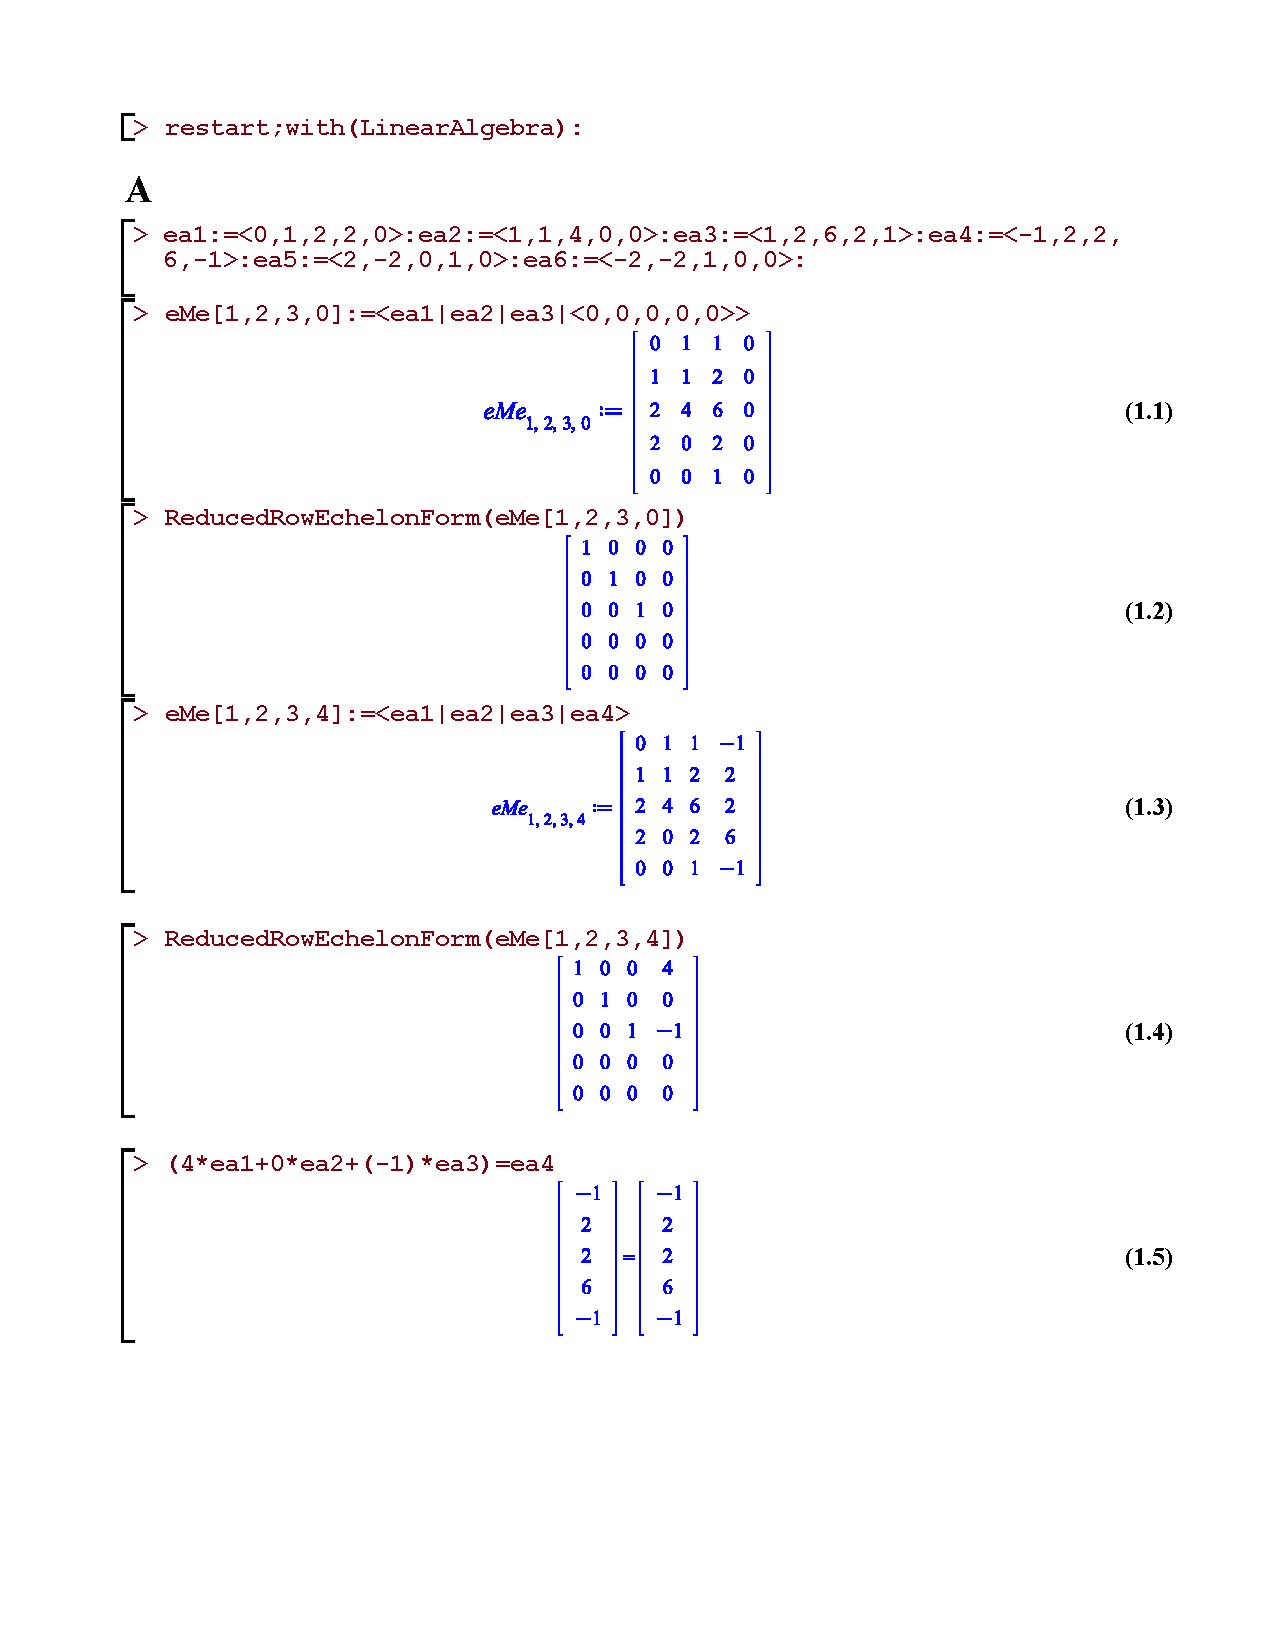
\includepdf[pages=1,pagecommand=\section{Appendiks}]{Opgave 3.pdf}
\includepdf[pages=2-]{Opgave 3.pdf}




